\chapter{Existing solutions}

There are many existing game engines, and it is important to examine where they succeed and where they fail. Sadly, as I have mentioned there aren't many engines that we can use for free, and there are even fewer engines where we can see the source code as well. In this section I will be presenting a few of the existing engines and what I think their strong points and mistakes are.
As I have the most experience with Unity I will be exploring it in more detail than the others.

\section{Unity}

The Unity game engine\cite{unity}, developed by Unity Technologies, is an extensive platform known for creating a many types of interactive content, with a primary emphasis on video games. But it is also used in simulations, or architectural visualization. This engine allows the creation of 2D, 3D, and virtual reality (VR) games, for almost every platform such as Windows, macOS, Linux, Mobile, and consoles. Unity rose in popularity due to its unparalleled cross-platform capabilities, easy to use environment, and the supportive community that formed around it. It uses C\# as the primary scripting language, which is known for its versatility and efficiency, this also made it popular among developers. Additionally, its intuitive design and the availability of extensive learning resources have made Unity highly accessible, propelling its popularity.

In Unity, the game's world - called Scenes - are built from Game Objects, which can represent anything that is necessary for the gameplay. Most commonly these include the player and the environment they are in, but can also be more abstract things like managers for different game systems. To give these Game Objects logic, the user needs to add Components to them. One of the most common component is a Mesh and Mesh renderer which make the Game Object show up in the game world. The engine has many other built in components that can add physics, rendering, sound and many other capabilities to the objects. If the built-in set of components are not enough, than the user can create custom components by writing C\# scripts that extend the MonoBehaviour base class. 

The game objects can be attached to each other called "parenting", this causes them to move together with the parent object. This is commonly used to make a camera or a weapon follow the player. These scenes are authored inside the editor using the Scene view, Hierarchy, and Inspector sections. In the scene view, we have a bird's eye view of the environment we are creating, while the Hierarchy and Inspector views provide a more abstract way of editing the scene. The Hierarchy shows a list of all the Game Objects that are present in the scene, as these can have parent-children relations this view forms a tree.

Despite Unity's popularity in the independent developer community and huge success in creating diverse games, it is not without shortcomings. One of the most glaring issues I have encountered have been with the sporadic updates. Unity seams to be focused on chasing the newest and most cutting edge technologies, but this often results in a neglect of existing bugs and stability issues. As a long time user, it feels like the engine has become more and more cluttered with new features, and even more bugs. Many of the new features announced years ago are still in development, and many others have been silently stopped in development. 

Because of this constant chase of the new technologies, there are many areas where there are many competing solutions for a single problem. The most infamous example is the networking solutions, where there are multiple solutions, or the same with the game UI. These make the developer's choice for what system to use harder, as the older solution might be unsupported in the next engine version but not ready in the current version. This makes even starting a new project really hard and need a lot of unnecessary decisions.

\begin{figure}[h]
    \centering
    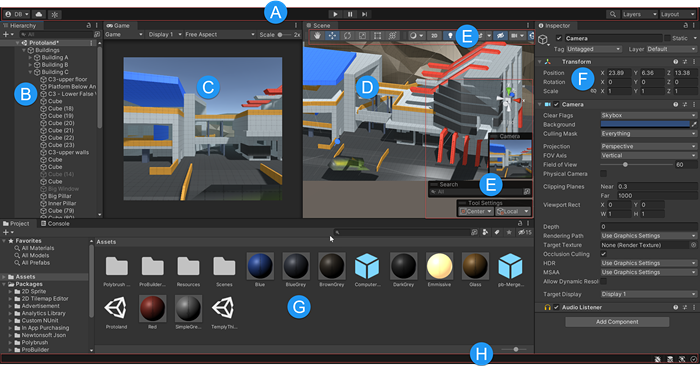
\includegraphics[width=0.5\textwidth]{content/002-research/unity-editor.png}
    \caption{The unity engine's editor with the major parts highlited}
\end{figure}


\section{Unreal Engine 5}

Unreal Engine, developed by Epic Games, has a rich and enduring history that has significantly influenced the landscape of modern gaming. The inception of Unreal Engine dates back to 1998, when the first-person shooter game 'Unreal' was released. Since then, it has undergone several mayor transformations, resulting in its latest iteration, Unreal Engine 5. Throughout the years, the engine has consistently pushed the boundaries of what's possible in game development, from pioneering high-fidelity graphics to orchestrating expansive virtual worlds.

Unreal Engine 5, boasts a tremendous leap forward in visual fidelity, my using groundbreaking technologies such as Nanite and Lumen. 
Nanite is a system that essentially eliminates the limitations of polygon count and draw call overheads in 3D environment modelling. It achieves this by using so-called "virtual polygons", allowing for much greater model detail to be used without major performance hit. This system can replace the traditional Level Of Detail (LOD)\footnote{A system where separate models are created for when the given object is further away.} approach, allowing for much faster development time.
Lumen, on the other hand, is a fully dynamic global illumination solution that can immediately react to scene and light changes, producing more lifelike environments. It is important to highlight that while these technologies can produce stunning visuals, they are slower than traditional approaches and not suitable for every game. 
